% !Tex root = main.tex

% agregator ako nastroj na koordinaciu distribuovanych, kontrolovanych nalozi.

%agregator must communicate efficiently the loads they control (called aggregate flexibility) to a system operator 
% small attention to communication of aggregator a system operator 


%maximum entropy feedback (MEF) - we get properties of it

%MEF is then used as a penalty in novel predictive control (PPC)

% PPC system advantages - modification of vanilla MPC

%No need for exact states and constraints of loads - only MEF is needed

% fast computation less number of variables than MPC 

% under certain regularity PPC is optimal

%Distributed energy resources (DER) refers to often smaller generation units that are located on the consumer's side of the meter. Examples of distributed energy resources that can be installed include: roof top solar photovoltaic units. wind generating units. battery storage.


%An independent and federally regulated entity that coordinates regional transmission to ensure non-discriminatory access to the electric grid and a reliable electricity system.


% by reinforcement learning aggregator can send flexibility (MEF) feedback

%aim of system operator (ISO) is to minize costs

%MEF should be general for various controllable loads:heating,air conditioning 
%power grid - energeticka siet

%%%%%PHD praca 
%straty na vedeniach - transmission loss

%First, they defined physical inefficiencies of power grids due to aging infrastructure – old wires, for example – as technical losses

%Next, they defined regulatory inefficiencies resulting in power consumption without financial compensation – such as fraud, meter tampering, and stealing – as non-technical losses, which can alter demand for electric power and thus its consumption patterns. These losses can be estimated (with uncertainty) from data for power generated, consumed, and paid for within each country.


%The proportion of technical to non-technical losses helps inform us of region-specific (rather than global) needs to lower emissions from T&D losses. For example, countries experiencing war and conflict, such as Haiti, Iraq, and Pakistan, suffer from some of the highest T&D losses in the world due to widespread destruction of their infrastructure. Without the resources to repair and reconstruct, these countries suffer from highly inefficient power grids and thus higher emissions that are not simple to address.


%Thus the goal is to design a model which derives the expected line
% losses from estimates on electrical supply, demand and exchange flows. The task is
% to increase the accuracy and precision of the existing line loss prediction method
% at Svk and reduce the existing error between actual and predicted line losses. The
% final objective is to provide recommendations on how to administer transmission
% line losses at Svk in the future. Thus, this thesis intends to complete the following
% aims:

%sucasny stav riesenia problematiky dopisat ako sekciu ako sa ten problem riesi
% co riesime prepisat lepsie nas sposob
% 

\chapter{Opis problému}
% \chapter{Opis problému.}

V tejto kapitole formulujeme problém, ktorý riešime a hovoríme aj o súčasnom stav jeho riešenia. Spomíname viacero prístupov od iných autorov, ktoré tento problém riešia.

% TODO: mozno viac dodat, ze ake obmedzenia atd, ale to mozno neskor

%V časti Súčasný stav riešenej problematiky doma a v zahraničí autor uvádza dostupné informácie a poznatky týkajúce sa danej témy. Zdrojom pre spracovanie sú aktuálne publikované práce domácich a zahraničných autorov. Podiel tejto časti práce má tvoriť približne 30 % práce.
% optimalny plan nabijania asi nie
\section{Formulácia problému.}
% optimálny nie lebo MPC offline je optimum a my hladame v online algoritmoch
Problém, ktorý riešime formulujeme takto:
Hľadáme plán nabíjania elektromobilov v nabíjacej sieti, ktorý zabezpečí maximálne dodávky požadovanej energie. Plán nabíjania musí dodržiavať obmedzenia nabíjacej siete. Obmedzenia, ktoré používame pri riešení problému sú:
% JPL ma tazsie obmedzenia zda sa 
\begin{enumerate}
    \item Jednofázové. Jednofázové obmedzenia infraštruktúry sú množinou linearných obmedzení. 
    \item Nevyvážené trojfázové. Nevyvážené trojfázové obmedzenia pozostávajú z množiny obmedzení kužeľa druhého rádu. Tento typ obmedzení má nabíjacia sieť Caltech ACN.
\end{enumerate}
Ďalšie parametre nabíjacej siete, ktoré pri riešení problému nastavujeme sú nabíjačky (ich počet a typ), transformátor (jeho kapacita). Musíme si zvoliť aj tarify (ceny nabíjania v čase). Viac informácii o obmedzeniach a parametroch sa nachádza v článkoch \cite{lee2021acnsim,Lee2018LargeScaleAE}.


Problém, ktorému sa venujeme je optimalizačným problémom, lebo hľadáme taký plán nabíjania, ktorý maximalizuje účelovú funkciu. 

% zarovnat tu pravu cast nejako

Formálnejšie definujeme tento optimalizačný problém takto:
$\overset{above}{main}$
% $\underset{\underset{r}{\max}}{SCH}$
\begin{align}
    \label{eq:utility-function-general}
    \overset{SCH}{\underset{r}{\max}} \; U_{k}(r) \\
    \text{subject to:} \\
    0 ≤ r_{i}(t) ≤ \overline{r}_{i}(t)  \qquad t < d_{i}, i ∈ V \\
    r_{i}(t) = 0 \qquad t ≥ d_{i}, i ∈ V \\
    \sum_{t = a_{i}}^{d_{i} - 1} r_{i}(t) \delta ≤ e_{i} \qquad i ∈ V \\
    f_{j}(r_{1}(t), \dots, r_{N}(t) ) ≤ R_{j}(t) \qquad t ∈ T, j ∈ \hat{R}
    % r \in R_{k}
\end{align}
$\hat{R}$
% napisat R so striezkou neviem ako to spravit
\ref{eq:einstein}

% sa snažíme maximalizovať množstvo dodanej energie elektromobilom. 












%  elektromobilom v nabíjacej sieti.










\section{Súčasný stav riešenej problematiky.}
Množstvo elektromobilov (okrem dvojkolových a trojkolových) sa má podľa predikcií \cite{iea2023} zvýšiť od roku 2022 do roku 2030 o 230 miliónov. Zvýši sa počet nielen súkromných elektrických aút, ale napríklad aj počet elektrických autobusov v mestskej hromadnej dopravne. \cite{iea2023} Veľa nabíjacích staníc dnes používa na nabíjanie elektromobilov plánovací algoritmus neriadeného nabíjania. Tento algoritmus sa už nebude môcť pri pribúdajúcom množstve elektromobilov použiť z dôvodu, že neberie do úvahy kapacitu nabíjacej stanice na energiu. \cite{lee2021acnsim} 

V poslednom desaťročí sa vedci snažili hľadať rôzne ďalšie algoritmy, ktoré by vedeli vyriešiť problém nabíjania elektromobilov pri zachovaní obmedzení infraštruktúry. \cite{iea2023} Potreby používateľov elektromobilov ako spotrebiteľov sú veľmi dôležité pri formulovaní optimalizačného problému, ktorý má tieto algoritmy riešiť.



My sa venujeme optimalizačnému problému dodania najväčšieho množstva požadovanej energie elektromobilom pri zachovaní obmedzení infraštruktúry siete. Riešením tohoto problému vieme zabezpečiť to, že nabíjané elektromobily získajú čo najväčšie množstvo požadovanej energie. 


% acnsim clanok 


% Neriadené nabíjanie, ktoré dnes veľa nabíjacích staníc pre elektrické vozidlá využíva na nabíjanie ele sa už nebude môcť  


\section{Súčasný stav riešenej problematiky v reálnom živote.}


Problematiku riešenia optimalizačného problému dodania najväčšieho množstva požadovanej energie elektromobilom pri zachovaní obmedzení infraštruktúry riešia v článkoch \cite{lee2021adaptivephd,Li_2021,chen2021smoothed}. 
Na riešenie tohoto optimalizačného problému sa v súčasnosti využíva neriadené nabíjanie, spomína sa v \cite{lee2021acnsim}. Jednou z komplikácii pri takomto riešení optimalizačného problému je, že môže dôjsť k preťaženiu infraštruktúry nabíjacej siete. Nižšie spomíname, ako tento optimalizačný problém riešia v literatúre, a ako ho riešime my. \cite{lee2021acnsim}


\section{Súčasný stav riešenej problematiky v literatúre.}

V dostupnej literatúre je veľa zaujímavých algoritmov, ktoré sa však nedájú využiť priamo v praxi. Hlavným dôvodom prečo sa nedajú aplikovať je poďla \cite{lee2021adaptivephd} to, že výchádzajú z predpokladov, ktoré v praxi nefungujú alebo im chýba schopnosť splniť praktické obmedzenia a ciele. 
% viac specifikovat prakticke obmedzenia a ciele

V článku \cite{Li_2021} tento problém rieši hlavne systémový operátor. Systémový operátor vyrieši optimalizačný problém, a tým získa množstvo energie, ktorú pošle agregátorovi.  Agregátor pomocou plánovacieho algoritmu získa plán nabíjania elektromobilov a dodá energiu elektromobilom.



My pri riešení tohoto optimalizačného problému využívame online plánovacie algoritmy s využitím balíka acnportal. Vstupom do online algoritmov sú elektromobily a ich parametre, ako napríklad čas ich príchodu, čas ich odchodu a ich požadovaná energia. Pomocou online plánovacích algoritmov získame poradie, v ktorom elektromobily nabíjame. Aby sme zistili množstvo energie, ktorú treba každému elektromobilu dodať, musíme vyriešiť spomínaný optimalizačný problém. Naším zámerom je riešiť optimalizačný problém osobitne pre každý elektromobil. Tento optimalizačný problém riešime metódou lineárneho vyhľadávania, metódy bisekcie, metódy dichotómie a pomocou kontrolných algoritmov (MPC). Riešením tohoto optimalizačného problému je optimálny plán nabíjania elektromobilov vzhľadom k dodanej energii.

% Riešenie tohoto optimalizačného problému v článku+
% pozriet ako toxin li v tom jeho clanku spominal podobne riesenia


%first sentences of the thesis strong and clear - to get interest of the reader
\chapter{Cieľ práce}

Cieľ práce je navrhnúť a overiť model agregátora flexibility pre zvolený typ prosumerov. To znamená, že musíme popísať ako agregátor flexibility kupuje energiu, a ako ju následne elektromobilom dodáva. Energiu agregátor flexbility bude dodávať elektromobilom na základe plánovacieho algoritmu, ktorý rieši optimalizačný problém.  Vyriešime optimalizačný problém dodania najväčšieho množstva energie elektromobilom pri zachovaní obmedzení infraštruktúry. Využívame pri riešení optimalizačného problému online plánovacie algoritmy (kontrolné alebo triediace), pričom vychádzame zo základných tried v balíku acn portal, ktoré definujú obmedzenia nabíjacej siete a zjednodušujú prácu s novo implementovanými algoritmami. Vstupom algoritmu, ktorý rieši tento optimalizačný problém sú údaje o príchodoch elektromobilov do nabíjacej siete Caltech. Výstupom tohoto algoritmu je celkový pomer dodanej požadovanej energie elektromobilom a celkové cena dodanej energie elektromobilom atď. Overíme si navrhnutý model agregátora flexibility na verejne dostupných vstupných dátach z Caltech nabíjacej siete.  








% \section{Činnosti agregátora flexibility}


\section{Úlohy agregátora flexibility}
V súčastnosti pozorujeme pokrok v oblasti distribuovania obnoviteľnej energie. S čoraz vyšším dopytom po energii sa vedci musia zaoberať výskumnou otázkou: Ako môžu spotrebitelia dodávať energiu a zároveň ju prijímať? To znamená, že treba zmeniť jednosmernú sieť, kde veľké firmy dodávajú energiu spotrebiteľom, na obojsmernú sieť, kde spotrebitelia dodávajú a zároveň prijímajú energiu (skrátene takých spotrebiteľov nazývame prosumeri). Vedci ako odpoveď na túto výskumnú otázku zaviedli novú kategóriu hráčov na trhu s energetikou. Túto novú kategóriu hráčov nazývame agregátori. 


Agregátor je prostredníkom medzi prosumermi a trhom s elektrinou, tým že združuje flexibilitu od prosumerov, a následne flexibilitu predáva (ako jedna entita) na trhoch s elektrinou. Prosumeri sú odmeňovaní za poskytovanie flexibility agregátorovi.

Rola agregátora zatiaľ nie je presne definovaná. Rola agrégatora môže byť určená tretou stranou alebo môže byť určená už učinkujúcim hráčom na trhu s elektrinou, ktorý má napríklad záujem použiť agregátor na doplňujúce veci.
%doplnujuce veci - vysvetlit

Nezávislý agregátor môže poskytovať jednu službu alebo viac služieb. Medzi služby agregátora patria agregovanie flexibility, dodávky energie spotrebiteľom a vyváženie dopytu a ponuky na trhoch s elektrinou. \cite{Granado2023}


% Systémy v elektrickej sieti môžu mat jeden centrálny agregátor alebo viac agregátorov.






% Prosumeri poskytujú agregátorovi svoju flexibilitu. 




% Agregátor má viacero úloh, ktoré rieši. Agregátor združuje elektrickú energiu od prosumerov. Agregátor pozoruje cenu energie na trhoch. Ak je cena energie veľmi vysoká, tak agregátor poskytuje spotrebiteľom menej energie. Naopak, keď je cena energie nízka, tak agregátor poskytuje spotrebiteľom viac energie.


% optional link

% https://en.energinet.dk/Electricity/Green-electricity/Demand-side-response/What-is-an-aggregator/

\begin{figure}[H]
    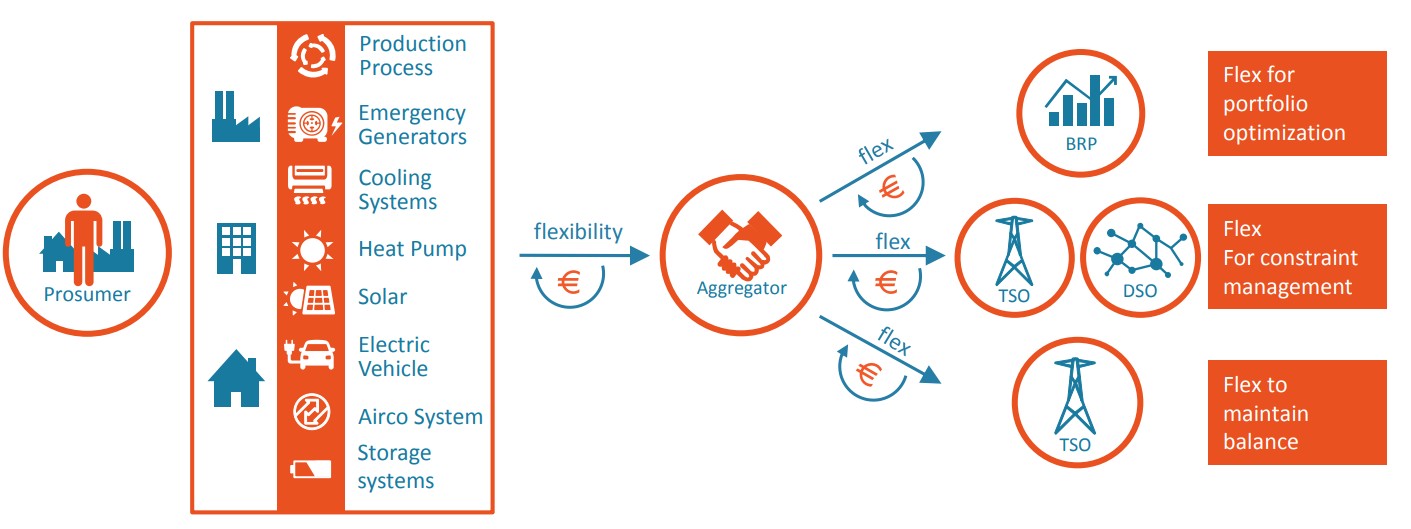
\includegraphics[width=\textwidth]{images/prosumers_aggregator.png}
    \centering
    \caption[Funkcie agregátora flexibility]{Distribúcia flexibility medzi prosumermi, agregátorom a trhom s elektrinou. Zdroj obrázka je \cite{usef2018}.}
    % \label{onlinealg:obrnotyet}
    \end{figure}


\UNFIN
% image source https://www.usef.energy/app/uploads/2016/12/USEF_IndependentAggregator.pdf

% \cite{KUBLI2021110908}

% \chapter{Východiská}
% \label{kapitola:vychodiska}
% V tejto kapitole popisujeme technologické a teoretické východiská, ktoré využívame v implementácii. Technologické východiská tvoria najmä Balíke, ktoré implementujú existujúce riešenia. Teoretické východiská zostávajú z veľkej časti podobné ako pri existujúcich riešeniach, aby sme vedeli následne efektívne porovnať našu implementáciu s existujúcimi riešeniami.


% \subsubsection*{Parametre spotrebiteľa.} 
% % \subsubsection*{Parametre spotrebiteľa} 

% Každému spotrebiteľovi $j = 1, \ldots, N$ je pridelená štvorica dát \\ $(a(j), d(j),  e(j), r(j)) \in R^{4}$. Parameter $a(j)$ znamená čas príchodu a parameter $d(j)$ je čas odchodu. Obe premenné sa normalizujú. Parameter $e(j)$ označuje množstvo požadovanej energie v jednotkách kWh a $r(j)$ je maximálne množstvo nabíjacej energie.

% \subsubsection*{Rozhodnutie agregátora.}
% % \subsubsection*{Rozhodnutie agregátora}
% Rozhodnutie agregátora v čase $t$ pre všetkých spotrebiteľov označujeme $s_{t}$. Premenná $s_{t}$ obsahuje pridelenie energie pre každého spotrebiteľa v čase $t$ na základe nejakého trediaceho algoritmu. Nech $\pi_{t}$ je použitý triediaci algoritmus (napr. Least Laxity First, Early Deadline First) v čase $t$. Potom premennú $s_{t}$ vypočítame takto:
% \begin{equation}
%     s_{t} = \pi_{t}(u_{t}),
% \end{equation}
% kde $u_{t} \in U$ je úroveň výkonu agregátnej rozvodne v čase $t$. 

% \subsubsection*{Stav agregátora.}
% % \subsubsection*{Stav agregátora}
% Stav agregátora v čase $t$ označujeme $x_{t}$. Hodnotu premennej $x_{t}$ zistíme takto:
% \begin{equation}
%     x_{t} = \{(d_{t}(j), e_{t}(j):a(j) < t < d(j)), j = 1, \ldots, N\},
% \end{equation}
% kde $e_{t}(j)$ je zostávajúca požadovaná energia a $d_{t}(j)$ je  zostávajúci čas na nabíjanie v čase $t$.

% \subsubsection*{Prechodové funkcie.}
% Každé rozhodnutie $s_{t}(j) \in R$ agregátora v čase $t$ pre spotrebiteľa $j$ zmení stav agregátora. Keď sa zmena aplikuje na všetkých spotrebiteľov stav agregátora sa zmení z $x_{t}$ na $x_{t + 1}$. Aplikujeme dve prechodové funkcie na $e_{t}(j)$ a na $d_{t}(j)$ takto:

% \begin{gather}
%     e_{t}(j) = e_{t - 1}(j) - s_{t}(j), \\ 
%     d_{t}(j) = d_{t - 1}(j) - \Delta,
% \end{gather}
% kde časový interval $\Delta$ je 12 minút. Predpokladáme, že nenastane žiadna strata energie. Tým dostaneme nový stav: 
% \begin{gather}
% x_{t + 1} = f(x_{t} \in X_{t}).
% \end{gather}  








% \subsubsection*{Podmienky pre rozhodnutie agregátora.}
% Podmienky, ktoré by mali byť rozhodnutím agregátora splnené sú:
% \begin{gather}
%     s_{t}(j) = 0, \text{ ak $t < a(j)$ alebo $t > d(j)$}, j = 1, \ldots N, \label{tv:pra:1} \\
%     \sum_{j = 1}^{N} s_{t}(j) = u_{t}, j = 1, \ldots N, \label{tv:pra:3} \\
%     \sum_{t = 1}^{T} s_{t}(j) = e(j), t = 1, \ldots T, \label{tv:pra:4}\\
%     0 \leq s_{t}(j) \leq r(j),t = 1, \ldots, T \label{tv:pra:5}.
% \end{gather}
% Obe podmienky~\ref{tv:pra:1} a~\ref{tv:pra:5} vždy platia. Dalšie uvedené podmienky nemusia nutne platiť.





% % \subsubsection{Maximum flexibility feedback.}
% % \subsubsection*{Maximálna odozva flexilibity.}
% % Nech $(p_{1}^{*}, \ldots, p_{n}^{*})$ je unikátne riešenie. Potom maximálnu odozvu entropie označujeme $p_{t}* = \psi_{t}(u_{t})$.

% % "Equation \ref{eq:quadratic} shows a quadratic function."




% % Operator vie naklady $(c_{1}, \dots, c_{n})$ a odozvu, ale nevie buduce naklady $(c_{i+1}, \dots, c_{T})$ a odozvu $(p_{i+1}, \dots, p_{T})$.


% % \subsubsection{Algoritmus hlbokeho ucenia}
% % \begin{equation}
% %     j(\psi) = \sum_{t = 1}^{T}E [r(x_{t},p_{t}) + aH(\psi(x_{t}))]. \label{eq:Jahu}
% % \end{equation}

% % MSE 
% % \begin{equation}
% % MSE = \frac{\sum_{k = 1}^{L} \sum_{k = 1}^{T} |\sum_{j = 1}^{N} s_{t}^{(k)}(j)  - u_{t}^{k}|^{2}}{L \cdot T \cdot \Omega}. \label{eq:MSE}
% % \end{equation}

% \subsubsection{MPE.} Chyba mean percentage error, v skratke MPE je pomer nedodanej energie k dodanej energii (porušenie podmienky \ref{tv:pra:4}). Počíta sa vzorcom:
% \begin{equation}
% MPE = 1 - \sum_{k = 1}^{L} \sum_{t = 1}^{T} \sum_{j = 1}^{N} \frac{s_{t}(j)}{\sum_{j = 1}^{N}e_{j}},  \label{eq:MPE}
% \end{equation}
% kde MPE nadobúda hodnoty z intervalu $[0, 1]$.



